\documentclass{article}
\usepackage{amsmath}
\usepackage{graphicx}
\usepackage{mathtools} % for Aboxed inside align


\graphicspath{{./images/}}

\title{Unit 3}
\author{Strannik}
\date{2023 July - 2023 August}


\begin{document}
\maketitle
\section{Introduction to Multivariable Functions}
\begin{itemize}
  \item To graph a multivariable function, you must have 1 dimention more than the number of \underline{independent} variables
  \item In multivariable functions there will be only 1 dependent variable
  \item To graph the domain of a multivariable function, the domain must have the same dimention as the number of independent variables and an axis for each of those variables
  \item To graph a multivariable function:
  \begin{enumerate}
    \item Set $f(x,y) = z$
    \item Try to get a surface you know
    \item Or just use a computer
  \end{enumerate}
  \item \textbf{Level curves} are the shapes we get when a plane intersects a surface at different \underline{levels} along the axis of the dependent variable
  \item A \textbf{contour plot} is a map of \underline{level curves}
  \item To graph contour plots:
  \begin{enumerate}
    \item Set $f = k$
    \item Manipuate the equation but as if $k$ isn't your dependent variable but rather a constant, so group it with other constants
    \item Plug in \underline{easy} numbers into $k$ to get your level curves
  \end{enumerate}
\end{itemize}


\section{Limits \& Continuity of Multivariable Functions}
\begin{itemize}
  \item For 1 variable functions it is easy to find limits because you only need to check if the values the curve is approaching from left and right are \underline{equal}
  \begin{align}
    \lim_{x \to a^{-}} f(x) = \lim_{x \to a^{+}} f(x)
  \end{align}
  \item For 2 variable function, however, you can't do this, since you have a surface instead of a curve, so there are \underline{infinite} paths approaching the point
  \begin{itemize}
    \item To prove a limit exists, you must prove that \underline{all} (infinite) paths are approaching the same point (\textbf{Squeeze Theorem} can be used)
    \item Also you can prove that a limit does \underline{not} exist by showing that along 2 paths we get a different value as we approach the same point:
    \begin{enumerate}
      \item Try $x = 0$ and $y = 0$ first
      \item If that didn't prove the limit D.N.E., choose other paths
      \item Try to substitute (something like $y = x$) into the limit so that the \underline{degrees} of the numerator and denominator are the \underline{same} (this is checking other path)
      \item Make sure to \underline{include the point} from the limit on your path
      \item Always use $x = 0$ or $y = 0$ as one of your paths/substitutions, if you can
    \end{enumerate}
  \end{itemize}
  \item For 3 variable function, paths are now \underline{parametric} ($t$ variable)
  \begin{itemize}
    \item You can prove the limit D.N.E. just like with 2 variable function:
    \begin{enumerate}
      \item Making sure the substituted path includes your point is also crucial
      \item Always choose an axis as one of your paths (make other axes = 0), if you can
      \item Substitution similar, but now it is making the function in terms of $t$
    \end{enumerate}
  \end{itemize}
  \item \textbf{Continuity}: a function is continuous at \underline{any} point on the region for which it is defined (domain)
  \begin{enumerate}
    \item Polynomials are continuous everywhere
    \item Rational functions are continuous everywhere the denominator does not eqal to 0
    \item Continuity holds for compositions
  \end{enumerate}
\end{itemize}


\section{Derivatives of Multivariable Functions}
\begin{itemize}
  \item To find the slope of a tangent line to a surface at a point, you must give the tangent line a direction, since there are infinite tangent lines at any point on a 3D surface
  \begin{itemize}
    \item Fully directional derivatives will come later
    \item For now the directions are restricted to the $y$-direction and $x$-direction
    \item To find the slope of tangent line in $x$-direction, contain the tangent line in a plane parallel to the $xz$-plane ($y$ is held constant)
    \item For $x$-direction hold $x$ constant (parallel to $yz$-plane)
  \end{itemize}
  \item The idea of treating a variable as a constant and thereby insuring that the tangent line is in the direction of the other variable is called \textbf{partial derivative}
  \begin{itemize}
    \item For a function $f(x,y) = z$, $\frac{\partial f}{\partial x}$ gives slope of the tangent line at a point in $x$-direction by holding $y$ constant (partial derivative with respect to $x$)
    \item Similarly, $\frac{\partial f}{\partial y}$ is partial derivative with respect to $y$
    \begin{align}
      \begin{split}
        \frac{\partial f}{\partial x} &= \frac{\partial z}{\partial x} = f_x = z_x \\
        \frac{\partial^2 f}{\partial x^2} &= f_{xx} \\
        \frac{\partial^2 f}{\partial y \partial x} &= f_{xy}
      \end{split}
    \end{align}
    \item Note the order of variables in different notations: $f_{xy}$ is the second derivative, where first was with respect to $x$, but second is with respect to $y$, while in $\frac{\partial f}{\partial x \partial y}$ the order is opposite
    \item Also, for any function continuous on a region, \textbf{mixed partial derivatives} are eqaul (just make sure you have the \underline{same letters})
    \begin{align}
      f_{xy} = f_{yx}
    \end{align}
  \end{itemize}
  \item In \textbf{implicit derivatives} of multivariable functions $z$ is imiplicitly defined variable, not $y$
  \begin{itemize}
    \item Don't forget to take derivatives of \underline{both sides}
    \item $z = f(x,y)$ so for $z\cdot x$ or $z\cdot y$ use product rule, but for $x\cdot y$ you will never use it since one of them will always be treated as a constant
  \end{itemize}
  \item \textbf{Laplace Equation:}
  \begin{align}
    \frac{\partial^2 f}{\partial x^2} + \frac{\partial^2 f}{\partial y^2} = 0
  \end{align}
  \begin{itemize}
    \item Problems will ask you if a given function satisfies this equation
  \end{itemize}
\end{itemize}


\section{Differentials}
\subsection{Differentials In 2D}
\begin{figure}[h]
  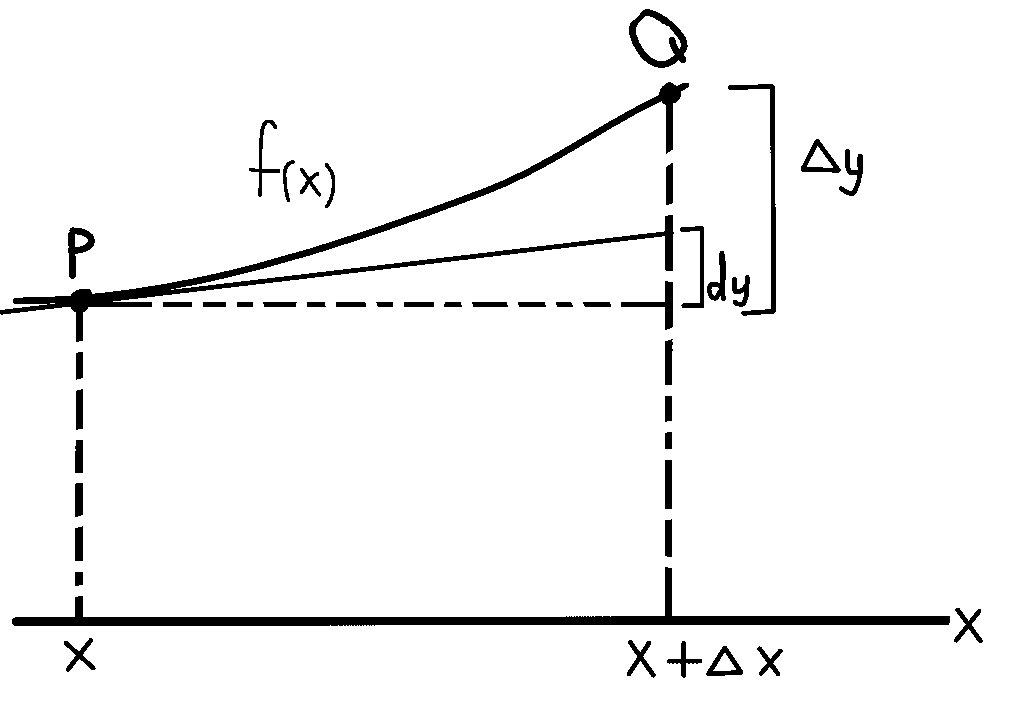
\includegraphics[scale=0.8]{differential-explained}
  \centering
  \caption{$dx = \Delta x$, $dy \neq \Delta y$}
  \label{fig:differential-explained}
\end{figure}
\begin{itemize}
  \item As $\Delta x$ gets really small ($\Delta x \to 0$), $\Delta y \approx dy$
  \begin{itemize}
    \item $\Delta y$ is increment
    \item $dy$ is differential
  \end{itemize}
  \begin{align}
    dy = f'(x)dx
  \end{align}
\end{itemize}

\subsection{Differentials of Multivariable Functions In 3D}
\begin{itemize}
  \item Because $x$ and $y$ are independent variables, $\Delta x = dx$, and $\Delta y = dy$
  \item However, it is different for the dependent variable $z$ (just like for $y$ in 2D):
    \begin{align}
      \Delta z \approx dz = f_x dx + f_y dy
    \end{align}
\end{itemize}

\subsection{Linearization}
\begin{itemize}
  \item Linearization is just making a linear function at a point and with the same slope as the multivariable function
  \begin{align}
    L(x,y) = f(x_0,y_0) + f_x(x_0,y_0)(x - x_0) + f_y(x_0,y_0)(y - y_0)
  \end{align}
\end{itemize}

\subsection{Error}
\begin{itemize}
  \item Max error: $|dz|$ (plug in $\pm$ error into $dx$ and $dy$)
  \item Max \% error: $\left| \frac{\Delta f}{f} \right| \approx \left| \frac{df}{f} \right|$
  \item You can also find error with this (\textbf{I don't know if it is the same error though}):
  \begin{align}
    |E| \leq \frac{1}{2}M\left( |x - x_0| + |y - y_0| \right)^2
  \end{align}
    \begin{itemize}
      \item To find $M$, take second derivatives $f_{xx}$, $f_{xy}$, $f_{yx}$, and $f_{yy}$, evaluate each at a point, then compare their absolute values, the greatest will be $M$
      \item $|x - x_0|$ and $|y - y_0|$ are usually given
    \end{itemize}
\end{itemize}


\section{Chain Rule for Multivariable Functions}
\begin{itemize}
  \item $y = f(x)$, $x = g(t)$ is a \underline{composition} and its derivative is:
  \begin{align}
    \frac{dy}{dt} = \frac{dy}{dx}\cdot\frac{dx}{dt}
  \end{align}
  \item \textbf{Intermediate variables} give you a pathway from the dependent variable to the independent variable ($x$ is an intermediate variable in this example)
  \item $t$ is the only independent variable, even if you have $x$, $y$, and $z$
  \item For a multivariable composition like $w = x^2 - y^2$, $x = t^2 + 1$, $y = t^3 + t$ the derivative is:
    \begin{align}
      \frac{dw}{dt} = \frac{\partial w}{\partial x}\cdot\frac{dx}{dt} + \frac{\partial w}{\partial y}\cdot\frac{dy}{dt}
    \end{align}
  \item If you have more than one independent variables (not intermediate), for example $u$ and $v$, do this for derivative:
  \begin{align}
    \begin{split}
      \frac{\partial w}{\partial u} = \frac{\partial w}{\partial x}\cdot\frac{\partial x}{\partial u} + \frac{\partial w}{\partial y}\cdot\frac{\partial y}{\partial u} \\
      \frac{\partial w}{\partial v} = \frac{\partial w}{\partial x}\cdot\frac{\partial x}{\partial v} + \frac{\partial w}{\partial y}\cdot\frac{\partial y}{\partial v}
    \end{split} \label{chain-partial-deriv}
  \end{align}
  \item A new way to do implicit differentiation when you have $w = f(x,y)$, $y = g(x)$
  \begin{align}
    \frac{dy}{dx} = -\frac{f_x}{f_y}
  \end{align}
  \begin{itemize}
    \item Note that in this equation, partial derivative with respect to independent variable is on top, while dependent variable derivative is on bottom (denominator)
    \item It can also work when you have multiple independent variables, similar to equations number \ref{chain-partial-deriv}
  \end{itemize}
\end{itemize}


\section{Directional Derivatives}
\begin{itemize}
  \item Partial derivativs are a kind of directional derivatives
  \item Directional derivatives give you slope at any point on a surface but only in the \underline{direction} of $\hat{u}$ (unit vector), which lies on the plane of independent variables ($x$ and $y$)
  \begin{align}
    D_{\hat{u}}f(x,y) = f_xu_1 + f_yu_2
  \end{align}
  \item $D_{\hat{u}}$ gives you slope, it is a scalar, not vector
  \item $\nabla$ symbol means \textbf{gradient}, which relates to the grade ("climb") of the surface
  \begin{align}
    \nabla f(x,y) &= f_x\hat{i} + f_y\hat{j} \\
    D_{\hat{u}}f(x,y) &= \nabla f(x,y)\cdot\hat{u}
  \end{align}
  \begin{itemize}
    \item $\nabla f$ is a vector (part of $D_{\hat{u}}$)
    \item If $\nabla f = 0$, then $D_{\hat{u}} = 0$ for any $\hat{u}$
    \item $D_{\hat{u}}(x,y)$ has its max value of $\|\nabla f(x,y)\|$, but only when $\hat{u}\parallel\nabla f$ (same direction), $\hat{u} = c\cdot\nabla f$ ($c$ is a scalar) and its min value is $-\|\nabla f(x,y)\|$
    \begin{align}
      D_{\hat{u}}f(x,y) &= \|\nabla f(x,y)\|\cos(\theta)
    \end{align}
    \item Where $\theta$ is the angle between $\nabla f$ and $\hat{u}$: when $\theta = 0$ slope is steepest, $\theta = \pi$ slope is min
    \item $\nabla f$ gives a vector for the steepest grade of a surface at a point
  \end{itemize}
\end{itemize}


\section{Tangent Planes \& Normal Lines}
\begin{itemize}
  \item On contour plots, the fastest way up a "hill", $\nabla f$, is the path $\perp$ to a level curve
  \begin{itemize}
    \item $\nabla f(x,y)$ gives normal to a level curve of $f(x,y) = c$
    \item $\nabla f(x,y,z)$ gives normal to a level \underline{surface} of $f(x,y,z) = c$
  \end{itemize}
  \item To find a normal for a 2D curve at a point:
  \begin{enumerate}
    \item Pretend the given equation is a level curve to a 3D surface
    \item Make a \underline{3D function} from your given equation's side with variables (left side of $x^2 - y^2 = 16$) or write $f(x,y)$ instead of the constant (because a level curve is $f(x,y) = c$)
    \item Find gradient of your made up function (that should look something like $f(x,y) = x^2 - y^2$)
    \item Plugging in a point into the gradient will give you the level curve's normal at this point (any point and any level curve of your made up surface will work)
    \item You can also do the same for a 3D surface to find its normal at some point, but then with the normal you can create a \underline{tangent plane}
  \end{enumerate}
\end{itemize}


\section{Extrema of 2 Variable Functions}
\begin{itemize}
  \item Relative max for a 2 variable function is a peak of a surface (unlike absolute max, there can be more than 1)
  \item Relative maxes and mins are given by \textbf{critical points} \underline{only}, but for 2 variable functions to have a relative extrema at the point: $f_x = f_y = 0$ and \underline{both} must be changing from $-$ to $+$ or vice versa
  \begin{itemize}
    \item Critical points of 2 variable functions can be \textbf{saddle points} ($f_x$ is changing from $-$ to $+$, while $f_y$ is changing from $+$ to $-$) or undefined (undefined partial derivative \underline{on function's domain})
    \item At critical points of 1 variable functions $f'(x) = 0$ or $f'(x)$ is undefined and also critical points can be points of inflection
    \end{itemize}
  \item Second derivative test tells you whether the critical point is a relative min or relative max
  \begin{align}
    D(x,y) = f_{xx}(x,y)\cdot f_{yy}(x,y) - (f_{xy}(x,y))^2
  \end{align}
  \begin{itemize}
    \item If $D(a,b) > 0$, your critical point is either a relative min or a relative max
    \begin{itemize}
      \item In this case both $f_{xx}(a,b)$ and $f_{yy}(a,b)$ have the same sign, so you only have to check one
      \item When you check $f_{xx}(a,b)$ or $f_{yy}(a,b)$: positive is concave up (relative min), negative is concave down (relative max)
    \end{itemize}
      \item If $D(a,b) < 0$, then $(a,b)$ is a \underline{saddle point}
      \item $D(a,b) = 0$ tells you nothing, \underline{inconclusive}
    \end{itemize}
  \item For \underline{absolute} min and max to exist, there must be a closed region on which $f(x,y)$ is continuous
  \begin{itemize}
    \item They must occur at either critical points or on the boundary of the region
    \item There can only be one value for absolute max and one value for absolute min, but there can be multiple point's at which they occur
    \item So to find your absolute min and max:
    \begin{enumerate}
      \item Draw the region's boundaries
      \item Find all \underline{relative} mins and maxes and their values
      \item Make equations for curves along your boundaries (substitution) and find where their derivatives = 0 (use those points \underline{only} if they are inside the region)
      \item Plug in those points along with the end points of the boundaries (corners of the rectangle or the triangle) into original equation
      \item Compare the values you get: greatest is absolute max, lowest is absolute min
    \end{enumerate}
  \end{itemize}
\end{itemize}


\section{Optimization \& LaGrange Multipliers}
\begin{itemize}
  \item When doing optimization problems:
  \begin{enumerate}
    \item You will have 2 equations: constraint and formula that you will maximize or minimize
    \item Use the constraint to make a substitution
    \item Take partial derivatives of the formula, make them = 0 and solve
    \item Do substitution and you will get the value of one of the variables
    \item Then make your way backwards up to the constraint equation to get the rest values of the variables
  \end{enumerate}
  \item LaGrange multiplier is $\lambda$
  \begin{align}
    \nabla f(x,y) = \lambda\nabla g(x,y)
  \end{align}
  \begin{itemize}
    \item To find $g(x,y)$ from given level curve, do the same you did while finding tangent plane: just replace the lonely constant on one side with $g(x,y)$
    \item Extrema will be found at the points that are solution to this equation
    \item You can do optimization using this trick ($g(x,y)$ is going to be the constraint)
  \end{itemize}
\end{itemize}
\end{document}
